\documentclass[11pt]{article}
\usepackage{setspace}
\setstretch{1}
\usepackage[T1]{fontenc}
\usepackage{amsmath,amssymb, amsthm}
\usepackage{graphicx}
\usepackage{bm}
\usepackage[hang, flushmargin]{footmisc}
\usepackage[colorlinks=true]{hyperref}
\usepackage[nameinlink]{cleveref}
\usepackage{footnotebackref}
\usepackage{url}
\usepackage{listings}
\usepackage[most]{tcolorbox}
\usepackage{inconsolata}
\usepackage[papersize={8.5in,11in}, margin=1in]{geometry}
\usepackage{float}
\usepackage{caption}
\usepackage{esint}
\usepackage{url}
\usepackage{enumitem}
\usepackage{subfig}
\usepackage{wasysym}
\newcommand{\ilc}{\texttt}
\usepackage{etoolbox}
\usepackage{algorithm}
% \usepackage{algorithmic}
\usepackage[noend]{algpseudocode}
\usepackage{tikz}
\usetikzlibrary{matrix,positioning,arrows.meta,arrows}
\patchcmd{\thebibliography}{\section*{\refname}}{}{}{}

\makeatletter
\renewcommand{\@seccntformat}[1]{}
\makeatother


\begin{document}



\title{\textbf{EECS 340: Assignment 4}}

\author{Shaochen (Henry) ZHONG, \ilc{sxz517} \\ Yuhui ZHANG, \ilc{yxz2052}}
\date{Due and submitted on 03/19/2020 \\ EECS 340, Dr. Koyut{\"u}rk}
\maketitle

% % % % % % % % % % % % % % % % % % % % % % % % % % % % % % % % % %
% % % % % % % % % % % % % % % % % % % % % % % % % % % % % % % % % %
% % % % % % % % % % % % % % % % % % % % % % % % % % % % % % % % % %
\section{Problem 1}

\begin{figure}[H]
    \centering
    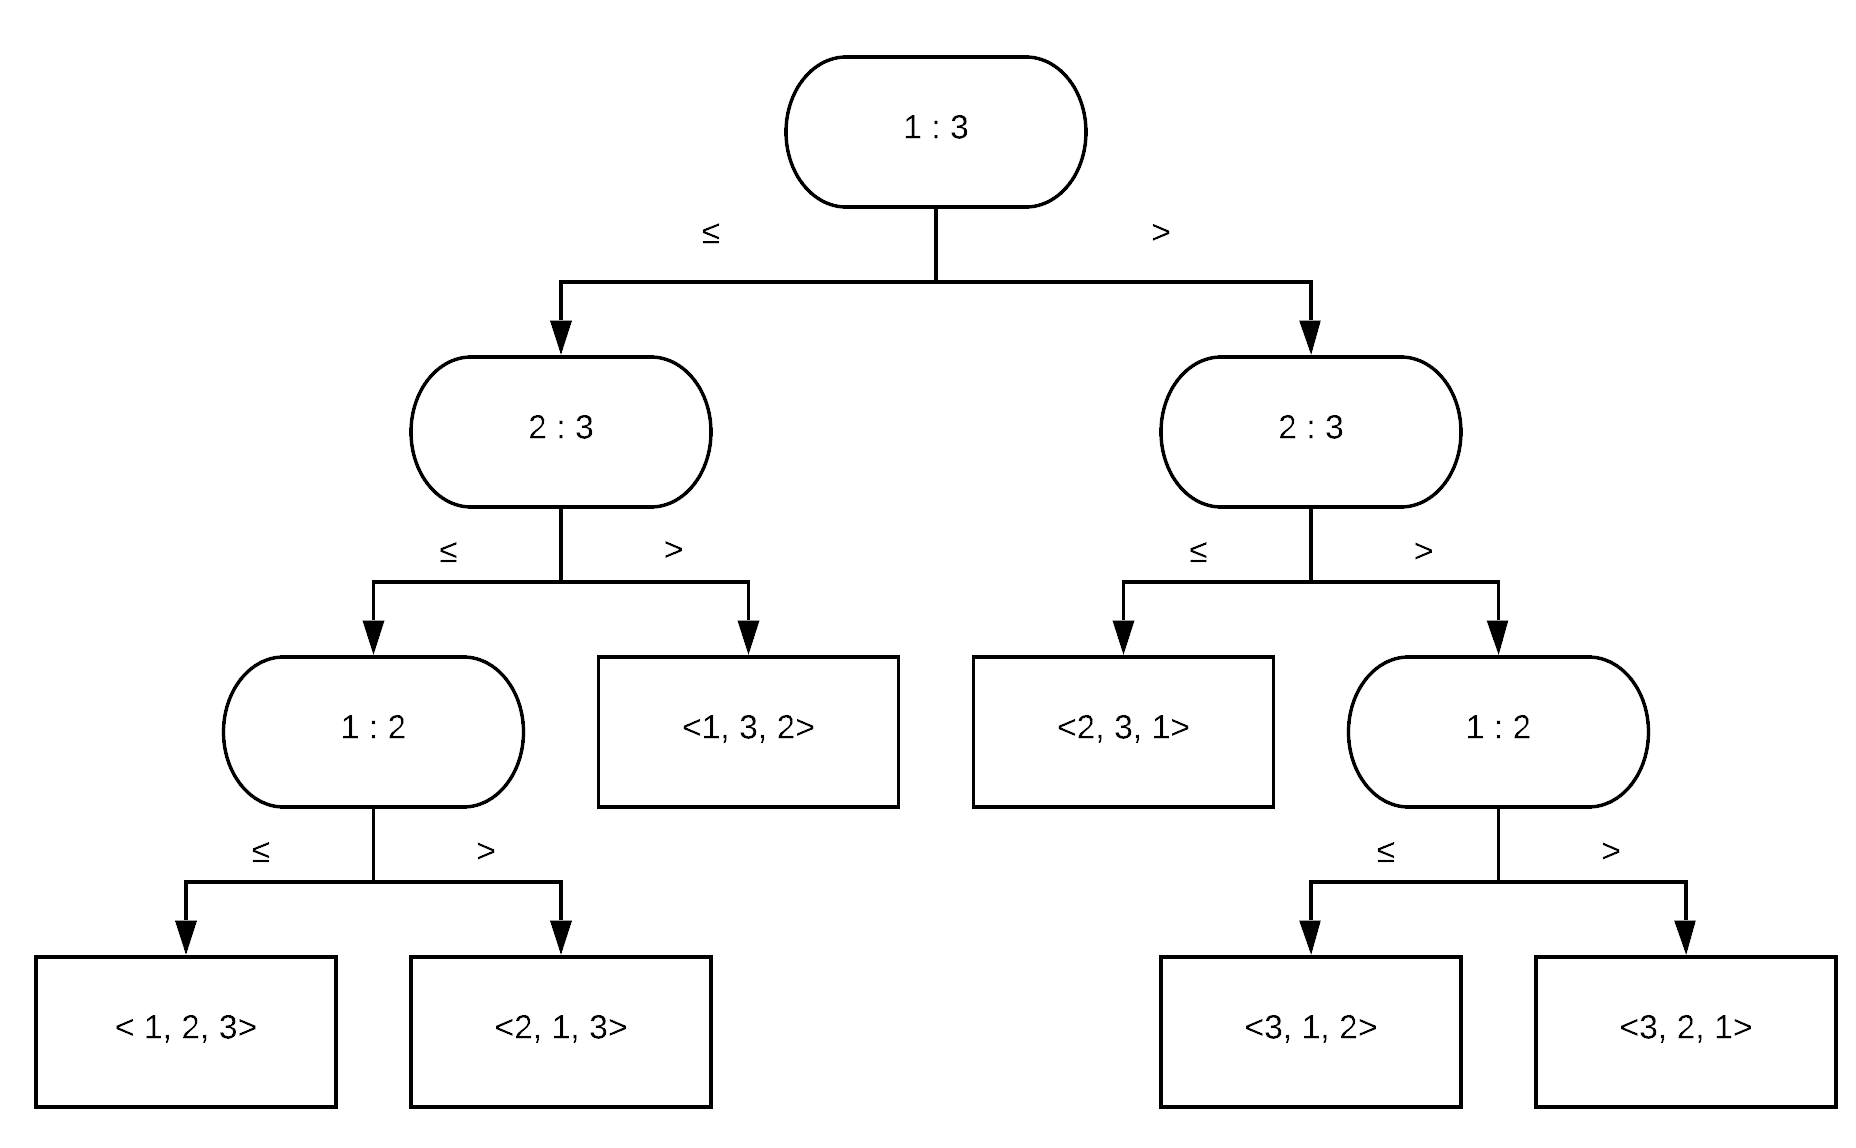
\includegraphics[width=0.8\linewidth]{{fig/fig_1.png}}
    \caption{Decision Tree of \textsc{Quicksort}}
    \label{fig:1}
\end{figure}

% % % % % % % % % % % % % % % % % % % % % % % % % % % % % % % % % %
% % % % % % % % % % % % % % % % % % % % % % % % % % % % % % % % % %
% % % % % % % % % % % % % % % % % % % % % % % % % % % % % % % % % %
\section{Problem 2}

\subsection{Procedure \textsc{PreProcess}(A)}

\begin{algorithm}
\caption{PreProcess(A)}\label{PreProcess}
    \begin{algorithmic}[1]
        \Procedure{PreProcess}{A, p, r}
        \State \text{Let $C[0, 1, ..., k]$ be an arry of $0$.}
        \For {$i \gets 0$ \textbf{to} $n$}
            \State $C[A[i]] = C[A[i]] + 1$
        \EndFor
        \For {$j \gets 1$ \textbf{to} $k$}
            \State $C[j] = C[j] + C[j-1]$
        \EndFor
        \State \Return $C$
        \EndProcedure
    \end{algorithmic}
\end{algorithm}

\subsection{Procedure \textsc{Query}(A, a, b)}

\begin{algorithm}
\caption{Query(A, a, b)}\label{Query}
    \begin{algorithmic}[1]
        \Procedure{Query}{A, a, b}
        \If {$a == 0$}
            \State \Return $A[b]$
        \Else
            \State \Return $A[b] - A[a-1]$
        \EndIf
        \EndProcedure
    \end{algorithmic}
\end{algorithm}

% % % % % % % % % % % % % % % % % % % % % % % % % % % % % % % % % %
% % % % % % % % % % % % % % % % % % % % % % % % % % % % % % % % % %
% % % % % % % % % % % % % % % % % % % % % % % % % % % % % % % % % %
\section{Problem 3}

% \section{References}
%
% \nocite{*}
% \raggedright
% \bibliography{references.bib}
% \bibliographystyle{plain}


\end{document}